\section{Evaluation}

We evaluated the timing compartments architecture using the gem5 architectural 
simulator~\cite{gem5} integrated with the DRAMSim2~\cite{DRAMSim2} memory 
simulator. Our experiments use multiprogram workloads comprised of SPEC2006 
benchmarks compiled for the ARM ISA. 

Table~\ref{tab:config} shows our system configuration.
The cores use the gem5 ``O3`` out-of-order core model which runs at 2GHz.  Each 
core has private 32KB L1 instruction and data caches, and private 256KB L2 
cache. The cores share a 4MB L3 cache. We derived cache configuration 
parameters from the Intel Xeon E3-1220L, which is a two core architecture used 
by Amazon EC2. In DRAMSim2, we simulate a 667MHz 2GB DDR3 memory. The 
interconnects in the simulator run at 1GHz. Unless specified otherwise, each 
experiment is fastforwarded for 1 billion instructions, and run for 100 million 
instructions. 

%We will first describe our security evaluation and then show
%the performance evaluation.

\begin{table}
    \caption{Simulator configuration parameters.}
    \centering
\begin{small}
    \begin{tabular}{|l|l|l|r|}
        \hline
        \multicolumn{3}{|l|}{gem5 core model} & ``O3''        \\\hline
        \multicolumn{3}{|l|}{CPU Clock}    & 2GHz             \\\hline
        \hline
        \multicolumn{2}{|l|}{Memory}             & 2GB    & 667MHz  \\\hline
        \hline
        \multicolumn{3}{|l|}{Network Clock}      & 1GHz \\\hline
        \hline
        L1d / L1i  & 32kB   & 2-way  & 2 cycles\\\hline
        L2         & 256kB  & 8-way  & 7 cycles \\\hline
        L3         & 4MB    & 16-way & 17 cycles  \\\hline
    \end{tabular}
    \end{small}
    \label{tab:config}
\end{table}

\subsection{Security}

At a high level, the general approaches that we use such as static partitioning,
duplication, and TDM should remove timing interference. We experimentally
tested the security to check if we missed any sources of timing interference.
We simulate a two-core 
system with two timing compartments, TC0 and
TC1, running concurrently. 
If there are no timing channels, then the execution time of a program on 
TC0 should be independent of the workload on TC1.
Using this reasoning, we verified the
security of our design by running, a fixed benchmark
on TC0 while varying the benchmark on TC1 and compared the execution times. 
As expected, 
we observed no interference with timing compartments enabled.

\subsection{Time Slice Coordination}
\label{sec:eval_coord}

The time multiplexed resources in this architecutre are interdependent, 
necessitating careful coordination among the time slices for each.
To explore a large design space of parameters (namely, the turn lengths and 
offsets) for the time slices for the TDM 
protected modules, we built a custom simulator that only models the memory
hierarchy for an L2 cache miss.
Given the turn lengths and offsets of each device, the L2 miss latency can
be determined based on the cycle in which an L2 miss happens.
Because a schedule repeats after the least common multiple of each turn length in 
the schedule multiplied by the number of timing compartments, each possible 
latency for a schedule can be enumerated. The simulator calculates
the expected value of the L2 miss latency assuming that distribution of L2 miss 
times is uniform random.

Using this simulator, we exhaustively tested the L2 miss latency for an
L3 hit under all possible turn lengths within wide search space (all turn 
lengths less than four times the greatest relevant latency in this subsystem),
and all possible offsets. The experiments confirmed that 
the intuitive schedule described in 
Section~\ref{sec:coordination} achieves the lowest expected L2 miss latency
assuming a hit in the L3 cache.
Fixing the turn lengths to the optimal values and adjusting only the offsets,
the worst case latency is 19.6\% higher than the one with the optimal schedule, showing
that coordinating TDM schedules is crucial.

The design space for schedules involving all resources from the L2 cache to
the main memory is far too large to search exhaustively.
Instead we used a simulated annealing otpimizer to search this design space.
First, we used the optimizer to study the L2 miss latency when the access misses
in the L3 as well.
After initializing the optimizer with the L3 miss schedule summarized in 
Table~\ref{tab:l2_miss_schedules}, the optimizer did not find a better schedule 
after 20,000 iterations. Fixing the turn lengths to those in the best
schedule and sweeping only the space of offsets,
the worst schedule we found had an average L2 miss latency that is 2.64X higher than the 
best schedule.

We used the same optimizer to find a schedule that minimizes the
L2 miss latency under the assumption that the L3 cache hit-rate is 90\%.
Optimizing for the L2 miss rate overall is a harder problem since it requires a 
balance bewtween the best L3 miss case and L3 hit case parameters. 
The schedule 
produced by the optimizer was not one that made any intuitive sense.  However, 
the optimal schedule was 39\% better than the worst schedule that used the 
same turn lengths as the best schedule (and as before, changed only the offsets).

The results for the schedule selection study are summarized in Table 
\ref{tab:coord_results}. Overall, scheduling interdependent time multiplexed 
devices is a challenging problem, but the gap between the worst and optimal 
cases show that it is important.

\begin{table}
    \caption{Scheduling Selection Study Results.}
    \begin{small}
    \centering
    \begin{tabular}{|l|l|l|l|}
        \hline
        \multicolumn{1}{|l|}{Optimized L2 Latency Case} & Search & Min & Max \\\hline
        \multicolumn{1}{|l|}{Assume L3 Hit} & Exhaustive & 25.5 & 30.5 
        \\\hline
        \multicolumn{1}{|l|}{Assume L3 Miss} & Simulated Annealing& 139.5 & 
        368.5 \\\hline
        \multicolumn{1}{|l|}{Assume 90\% L3 Hits} & Simulated Annealing& 38.1 & 
        53.1 \\\hline
    \end{tabular}
    \end{small}
    \label{tab:coord_results}
\end{table}

\subsection{Performance Overhead}

The timing compartments architecture extends the insecure baseline with
static partitioning and time multiplexing to secure the shared hardware 
resources. These changes lead to underutilization, and thus, a performance
overhead. To evaluate the performance overhead, we ran multiprogram workloads 
comprised of of SPEC2006 benchmarks, and measured the system throughput (STP).
% and the 
% average normalized turnaround time (ANTT).

STP is the throughput (in IPC) of the parallel system relative to the throughput 
of running each program serially. An STP of less than 1 means that higher 
throughput is achieved by running the programs serially rather than in 
parallel.
It is computed with
\begin{equation}
  \sum^n_{i=1} \frac{IPC_{MP,i}}{IPC_{SP,i}},
\end{equation}
where $IPC_{MP,i}$ is the IPC of the $i^{th}$ program in the workload when run 
in parallel with the others, and $IPC_{SP,i}$ is the IPC for the same program 
when it is run alone in the same system.

% ANTT is the average slowdown that each program experiences by running in 
% parallel with the others compared to running it alone. It can be calculated 
% using
% \begin{equation}
%   \sum^n_{i=1} \frac{T_{MP,i}}{T_{SP,i}},
% \end{equation}
% where $T_{MP,i}$ is the execution time of the $i^{th}$ program in the workload when run 
% in parallel, and $T_{SP,i}$ is the execution time for the same program 
% when it is run alone in the same system. STP and ANTT are similar, but do not 
% convey the same information. STP shows the performance from the perspective of 
% the system while ANTT shows the performance from the perspective of the user.

%We configured the security policy to disallow communication among all timing 
%compartments, and measured the execution time of the benchmark
%in TC0. 
Since the timing channel protection mechanisms primarily affect the 
memory hierarchy, the performance overhead heavily depends on the memory intensity 
of the benchmarks.
The memory intensity of each benchmark, in terms of L2 misses per thousand 
instructions, is shown in
Figure~\ref{fig:memstudy}. Of the SPEC2006 benchmarks, mcf has the most L2 misses,
while astar has almost none after fast-forwarding for 1B instructions.

\begin{figure}
    \begin{center}
        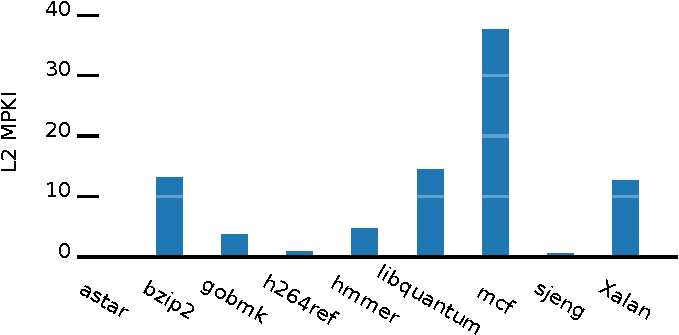
\includegraphics[width=3.4in]{figs/MPKI.pdf}
        \caption{Memory intensity of SPEC2006 benchmarks.}
        \label{fig:memstudy}
    \end{center}
\end{figure}

Table \ref{tab:workloads} summarizes the workloads we constructed to cover a 
variety of cases. For experiments with two cores, the workloads are exeactly as 
shown in the table. For experiments with more cores, the same labels are used 
to refer to workloads where half the cores run the first program, and the 
others run the second half. 
%% Consider commenting out the lines between this and the table
The first two letters indicate the memory intensity 
of each benchmark (low, moderate, or high). The letters "i" and "d" indicate 
that the performance of the benchmarks is largely independent or dependent on 
the cache size. The letters "p" and "n" indicate that the programs have phases 
or that they do not.

\begin{table}
    \caption{ Multiprogram Workloads }
    \centering
\begin{small}
    \begin{tabular}{|l|r|}
        \hline
        Workload Name & Benchmarks \\\hline\hline
        hhd &  mcf bzip2 \\\hline
        hhn &  mcf xalan \\\hline
        hhi &  libquantum libquantum \\\hline
        hli &  libquantum astar \\\hline
        hld &  mcf h264ref \\\hline
        hmi &  libquantum sjeng \\\hline
        hmd &  xalan gcc \\\hline
        mmi &  gcc gobmk \\\hline
        mmd &  sjeng sjeng \\\hline
        llp &  astar h264ref \\\hline
        lld &  h264ref hmmer \\\hline
        lli &  astar astar \\\hline
    \end{tabular}
    \end{small}
    \label{tab:workloads}
\end{table}

Figure ~\ref{fig:ntcstp} shows the STP of the insecure baseline (a) and of the 
secure processor (b) as the number of cores increases. The secure processor is 
configured so that each program runs in a separate timing compartment and no 
information leakage is permitted. The STP is greater than 1 for the secure 
processor for each workload and for each core count, showing that running in a 
shared system is beneficial even with a very strict security policy. Further, 
the STP of the secure processor with two cores is not significantly lower
than that of the insecure baseline. As the number of isolated programs 
increases, the overhead of the timing compartments scales linearly, but is
still reasonable.

\begin{figure*}%
  \begin{minipage}{1.2in}
    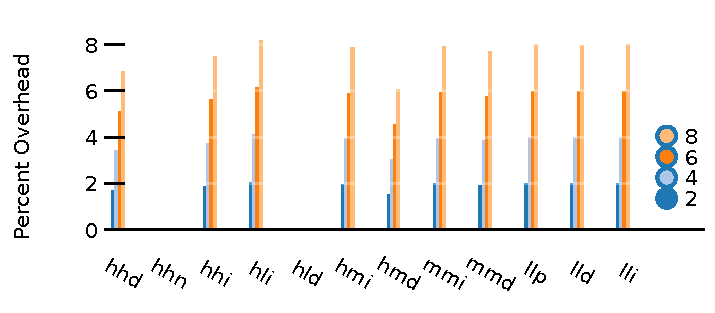
\includegraphics[width=3.4in]{figs/baseline_stp.pdf}
    \caption*{(a) Baseline}
  \end{minipage}
  \qquad\qquad\qquad\qquad\qquad\qquad\qquad\qquad\qquad
  \begin{minipage}{1.2in}%
        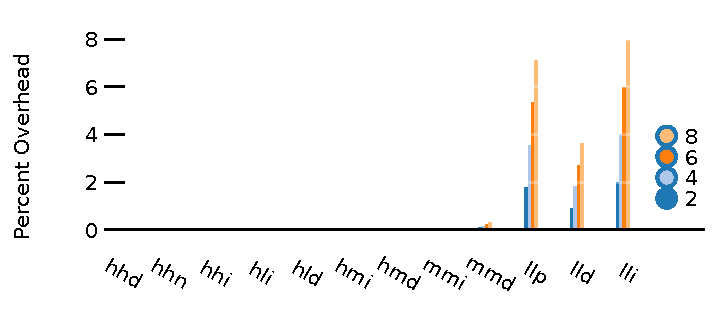
\includegraphics[width=3.4in]{figs/n_core_n_tc_stp.pdf}
        \caption*{(b) Secure}
  \end{minipage}%
  \caption{STP as the number of cores scales.} 
  \label{fig:ntcstp}%
\end{figure*}

Multiple programs can be grouped into the same timing compartment to allow 
resource sharing when permitted by the security requirements (for example, if 
two processes are owned by the same user or if some of the processes have low 
security needs). Figure ~\ref{fig:2tcstp} studies the performance gained 
through partial resource sharing by evenly dividing the processes in secured 2, 
4, and 6 core systems into two TCs. The performance gains are substantial and 
increase as the number of programs in the same TC increases.

\begin{figure}
    \begin{center}
        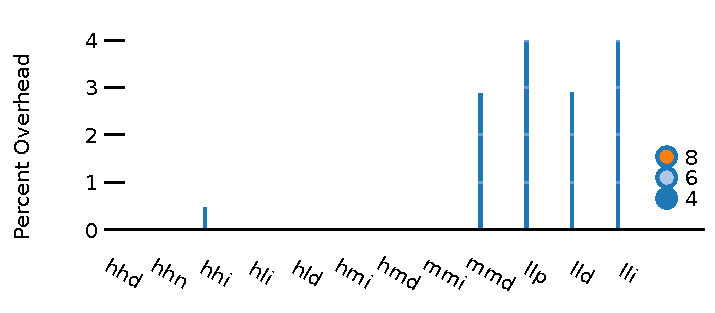
\includegraphics[width=3.4in]{figs/n_core_2_tc_stp.pdf}
        \caption{STP of systems with 2 TCs and more than 2 cores.}
        \label{fig:2tcstp}
    \end{center}
\end{figure}

In Figure ~\ref{fig:breakdown} we study the overhead of implementing each of 
the main protection mechanisms by evaluating the STP of a system with only 
cache way partitioning, the time multiplexed bus, or the time multiplexed 
memory controller. The results suggest that the majority of the overhead is due 
to the memory controller, and the cache partitioning and bus protection cause a 
much smaller portion of the overhead.

\begin{figure}
    \begin{center}
        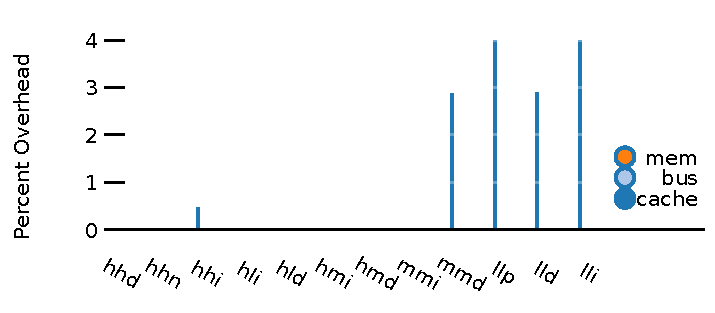
\includegraphics[width=3.4in]{figs/breakdown_stp.pdf}
        \caption{STP with individual security features enabled.} 
        \label{fig:breakdown}
    \end{center}
\end{figure}

In addition to these security features required for concurrently sharing the 
processor, TCs have an additional overhead whenever cores are shared by 
processes in different TCs through context switching. On a context switch, the 
private caches, shared cache partition, and the TLB and branch predictor state 
must be flushed. Figure ~\ref{fig:flushing} shows the STP of the secure system 
with context switches occuring every 1ms, 10ms, and 100ms. The overhead for 
context switching is not prohibitive, and we note that the additional overhead 
for context switching is only incurred on context switches between processes in 
different timing compartments. Context switches between processes within a VM, 
for example, will not have this overhead since they are most likely in the same 
TC.

\begin{figure}
    \begin{center}
        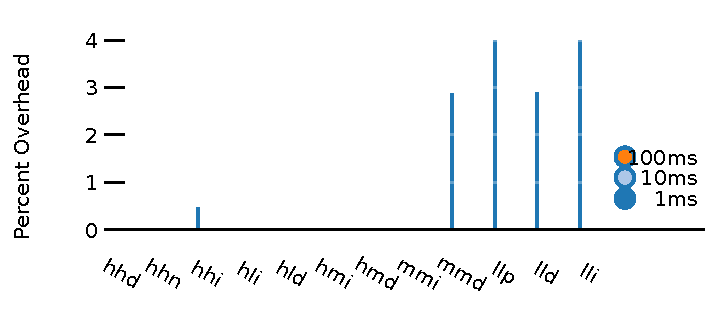
\includegraphics[width=3.4in]{figs/flushing_stp.pdf}
        \caption{Memory intensity of SPEC2006 benchmarks.}
        \label{fig:flushing}
    \end{center}
\end{figure}

\subsection{Cache Coherence Performance Overhead}

Adding the timing channel protection for snooping coherence bus can introduce 
performance overhead. We evaluate the overhead using SPLASH-2~\cite{splash2} benchmarks on 
gem5. The system we model is the one shown in Figure~\ref{fig:coherent_system}.
We use the same SPLASH-2 benchmarks for Attacker0 and Attacker1, each consists 
of two threads. We terminate the simulation
when thread on core 0 reaches 100M instructions.  Our baseline is a system 
where every other timing channel protection scheme we proposed is implemented 
except for the snooping bus.
We then compare it with the system where the snooping bus is also protected. 
This comparison enables us to quantify the overhead introduced by adding 
cache coherence protection. 

The results are shown in Figure~\ref{fig:splash2}. As can be seen, the overhead 
of adding cache coherence protection is
quite low, with the highest overhead less than 1.5\%. 
%In some cases the 
%protection scheme even outperform the baseline, mainly because the round-robin 
%scheduling may have avoided some snooping bus contention in the baseline 
%scheduling.  
The main reason for the low overhead is that the coherence protocol traffic 
is quite rare in programs, hence the TDM on the
snooping bus does not cause much overhead to the overall program execution 
time.

\begin{figure}
    \begin{center}
        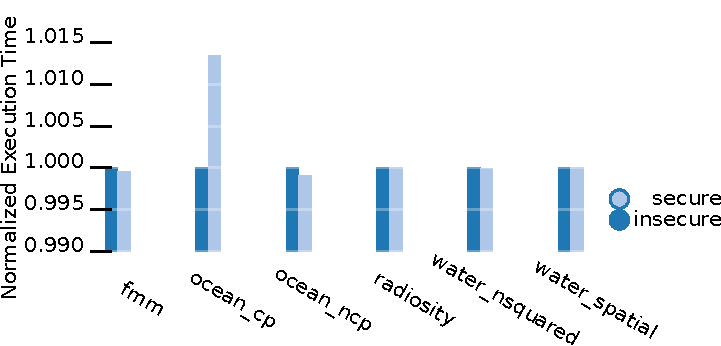
\includegraphics[width=3.4in]{figs/SPLASH.pdf}
        \caption{Performance overhead of cache coherence protection.}
        \label{fig:splash2}
		\vspace{-0.2in}
    \end{center}
\end{figure}
